\documentclass[12pt,a4paper]{article}

% --- Настройка языка и шрифтов для LuaLaTeX ---
\usepackage{fontspec}
\defaultfontfeatures{Ligatures=TeX,Scale=MatchLowercase}

\setmainfont{Alice-Regular}[
    Path=font/,
    Extension=.ttf,
    BoldFont = Alice-Regular,
    ItalicFont = Alice-Regular,
    BoldItalicFont = Alice-Regular,
    BoldFeatures = {FakeBold=1.6},
    ItalicFeatures = {FakeSlant=0.2},
    BoldItalicFeatures = {FakeBold=1.6,FakeSlant=0.2}
]

\newfontfamily\cyrillicfont{Alice-Regular}[
    Path=font/,
    Extension=.ttf,
    BoldFont = Alice-Regular,
    ItalicFont = Alice-Regular,
    BoldItalicFont = Alice-Regular,
    BoldFeatures = {FakeBold=1.6},
    ItalicFeatures = {FakeSlant=0.2},
    BoldItalicFeatures = {FakeBold=1.6,FakeSlant=0.2}
]

\usepackage{polyglossia}
\setmainlanguage{russian}
\setsansfont{TeX Gyre Heros}
\setmonofont{TeX Gyre Cursor}

\usepackage{graphicx}        					          % Графика
\usepackage[protrusion=false]{microtype}       	% Микротипографика
\usepackage{amsmath, amsfonts, amssymb, amsthm}	% Математика
\usepackage{braket} 							              % Braket нотация для квантовой механики
\usepackage{unicode-math} 						          % Современный пакет для математики в LuaLaTeX
\usepackage{longtable}       					          % Таблицы с разрывом страниц
\usepackage{tikz}           					          % Рисование
\usepackage[europeanresistors]{circuitikz}		  % Рисование электрических схем в европейском стиле
\usepackage{listings}							              % Для отображения кода
\usepackage{tabularx}       					          % Для таблиц во всю ширину
\usepackage{array}		  						            % Для расширенных возможностей таблиц
\usepackage{float}          					          % Для точного позиционирования фигур
\usepackage{pgfplots}                           % Для построения графиков
\usepackage{caption}                            % Для настройки подписей к рисункам и таблицам
\usepackage{xfp}                                % Для вычислений в LaTeX
\pgfplotsset{compat=1.18}
\usepackage[a4paper,left=20mm,right=20mm,top=20mm,bottom=20mm]{geometry}

\usetikzlibrary{arrows.meta}

% --- Колонтитулы ---
\usepackage{fancyhdr}
\pagestyle{fancy}
\fancyhf{}

\renewcommand{\headrulewidth}{0.4pt}
\renewcommand{\footrulewidth}{0.4pt}
\renewcommand\lstlistingname{Исходный код}

\lstdefinestyle{main}{
	backgroundcolor=\color{gray!8},   
	commentstyle=\color{green!50!black},
	keywordstyle=\color{blue!80!black},
	numberstyle=\small\color{darkgray},
	stringstyle=\rmfamily\color{orange!90!black},
	basicstyle=\ttfamily\small,
	breakatwhitespace=false,         
	breaklines=true,                   
	keepspaces=true,                 
	numbers=left,                    
	numbersep=8pt,                  
	showspaces=false,                
	showstringspaces=false,
	showtabs=false,                  
	tabsize=4
}	

\lstset{style=main}

\newcolumntype{C}{>{\centering\arraybackslash}X}
\renewcommand{\arraystretch}{1.25}

% =========================================================
%         СЛУЖЕБНЫЕ КОМАНДЫ ДЛЯ ВЫЧИСЛЕНИЙ
% =========================================================
\newcommand{\CalcTwo}  [1]{\fpeval{round((#1),2)}}
\newcommand{\CalcThree}[1]{\fpeval{round((#1),3)}}
\newcommand{\CalcFour} [1]{\fpeval{round((#1),4)}}
\newcommand{\CalcFive} [1]{\fpeval{round((#1),5)}}

\def\Discipline{Дифференциальные уравнения} % Название дисциплины
\def\LabTitle{Уравнение 2-ой степени}	    % Название лабораторной работы

\begin{document}

\fancyhead[L]{\LabTitle} 
\fancyhead[R]{\Discipline}
\fancyfoot[C]{\thepage}

\section{Решить задачу Коши
$$
y''-3y'+2y=5+e^x \quad y(0)=1 \quad y'(0)=0
$$}

\begin{center}
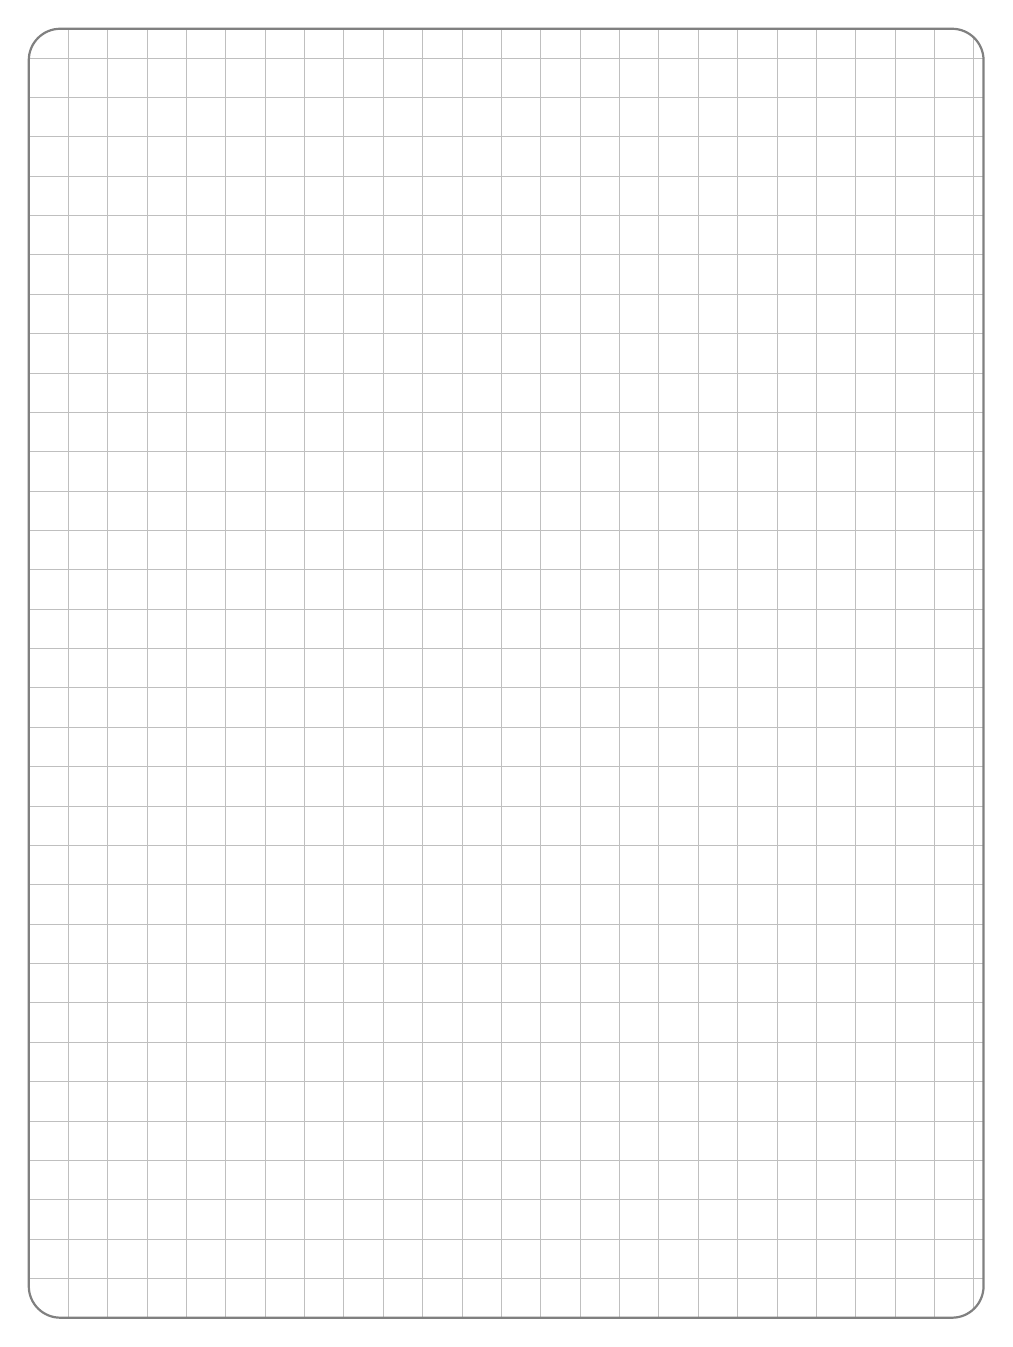
\begin{tikzpicture}
    % параметры
    \def\W{\textwidth}     % ширина прямоугольника
    \def\H{1.35\textwidth} % высота прямоугольника
    \def\R{4mm}     	   % радиус скругления
    \def\S{5mm}     	   % шаг сетки

    % обрезаем всё по прямоугольнику со скруглёнными углами
    \begin{scope}
        \clip[rounded corners=\R] (0,0) rectangle (\W,\H);

        % тетрадная сетка
        \draw[step=\S, very thin, gray!50] (0,0) grid (\W,\H);
    \end{scope}

    % внешний контур
    \draw[rounded corners=\R, line width=0.8pt, gray] (0,0) rectangle (\W,\H);
\end{tikzpicture}
\end{center}

\section{Решить задачу Коши
$$
y''-2y'+y=2 \quad y(0)=1 \quad y'(0)=0
$$}

\begin{center}
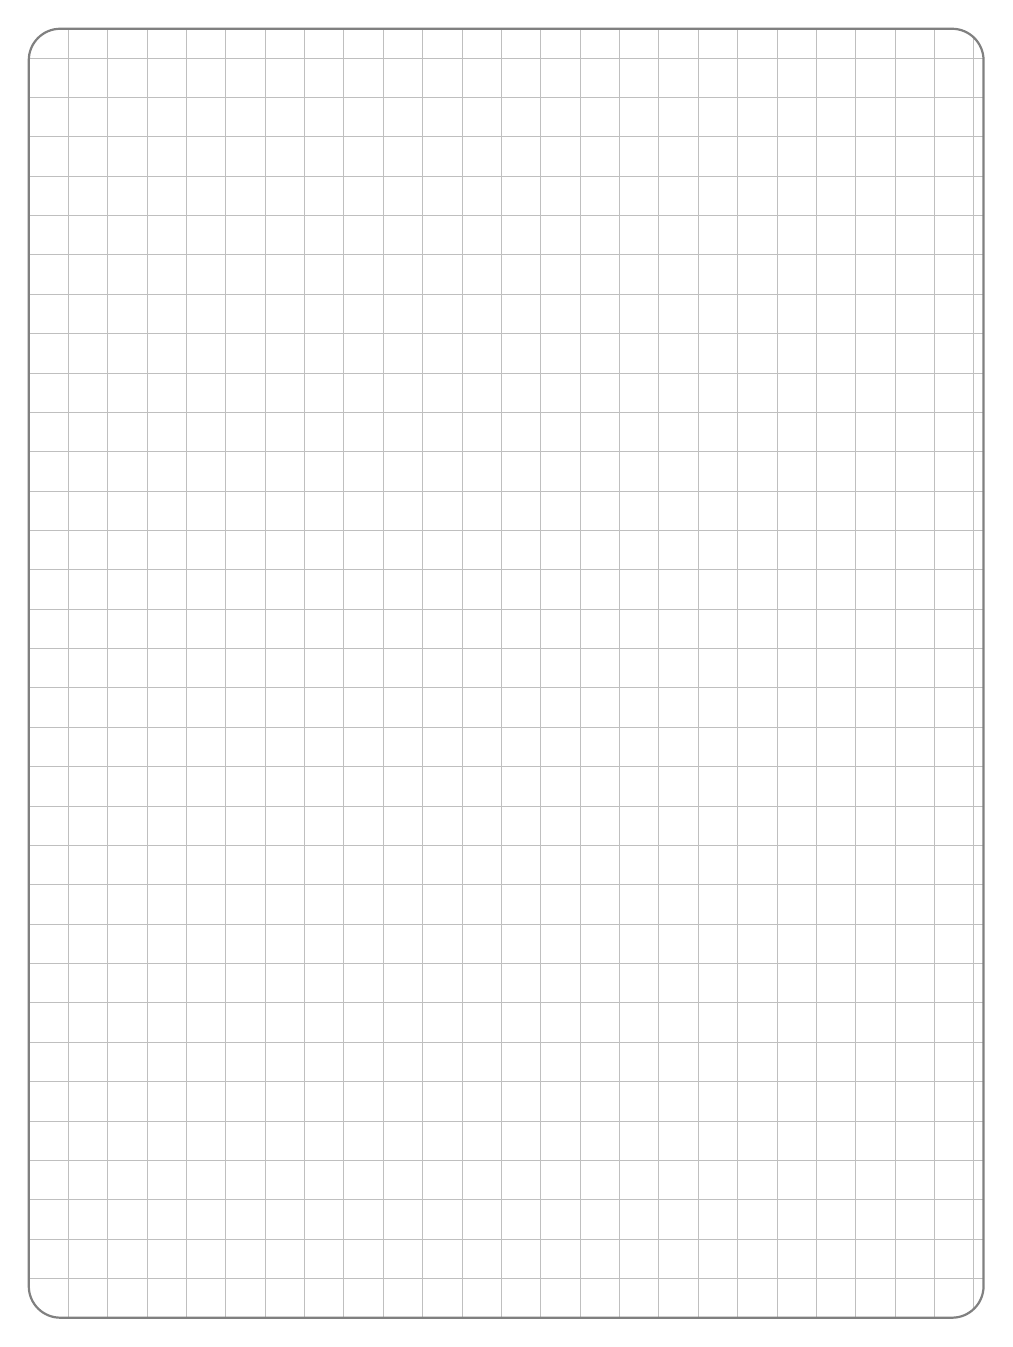
\begin{tikzpicture}
    % параметры
    \def\W{\textwidth}  % ширина прямоугольника
    \def\H{1.35\textwidth}       	% высота прямоугольника
    \def\R{4mm}     	% радиус скругления
    \def\S{5mm}     	% шаг сетки

    % обрезаем всё по прямоугольнику со скруглёнными углами
    \begin{scope}
        \clip[rounded corners=\R] (0,0) rectangle (\W,\H);

        % тетрадная сетка
        \draw[step=\S, very thin, gray!50] (0,0) grid (\W,\H);
    \end{scope}

    % внешний контур
    \draw[rounded corners=\R, line width=0.8pt, gray] (0,0) rectangle (\W,\H);
\end{tikzpicture}
\end{center}

\section{Решить задачу Коши
$$
y''+4y=\sin 2x + \cos 7x \quad y(0)=1 \quad y'(0)=0
$$}

\begin{center}
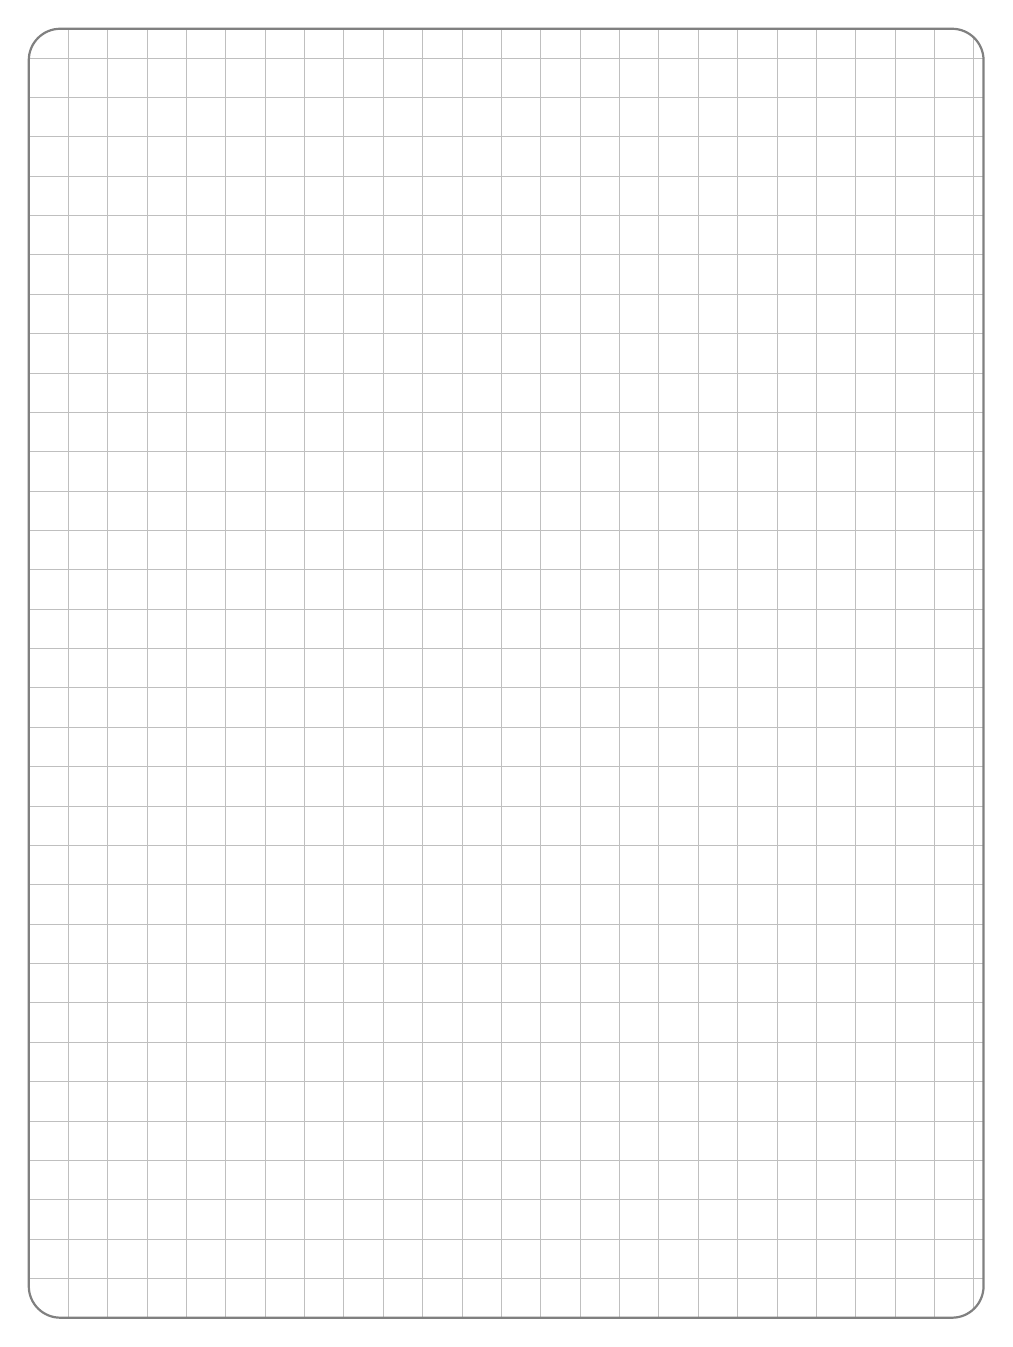
\begin{tikzpicture}
    % параметры
    \def\W{\textwidth}  % ширина прямоугольника
    \def\H{1.35\textwidth}       	% высота прямоугольника
    \def\R{4mm}     	% радиус скругления
    \def\S{5mm}     	% шаг сетки

    % обрезаем всё по прямоугольнику со скруглёнными углами
    \begin{scope}
        \clip[rounded corners=\R] (0,0) rectangle (\W,\H);

        % тетрадная сетка
        \draw[step=\S, very thin, gray!50] (0,0) grid (\W,\H);
    \end{scope}

    % внешний контур
    \draw[rounded corners=\R, line width=0.8pt, gray] (0,0) rectangle (\W,\H);
\end{tikzpicture}
\end{center}

\section{Решить задачу Коши
$$
y''+y=5\cos 2x - x\sin 2x \quad y(0)=1 \quad y'(0)=0
$$}

\begin{center}
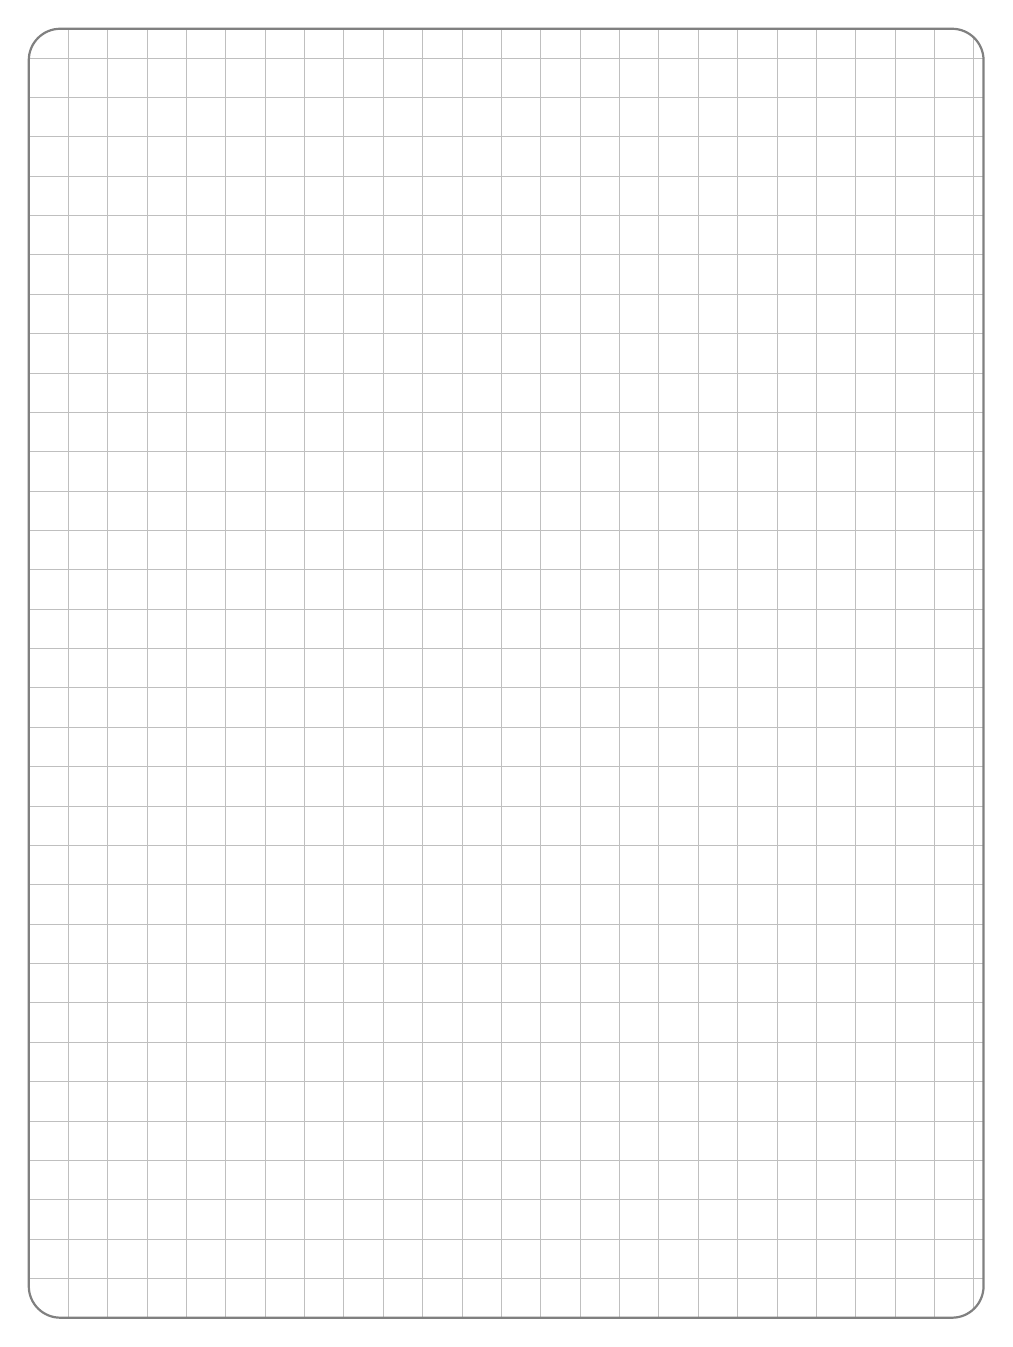
\begin{tikzpicture}
    % параметры
    \def\W{\textwidth}  % ширина прямоугольника
    \def\H{1.35\textwidth}       	% высота прямоугольника
    \def\R{4mm}     	% радиус скругления
    \def\S{5mm}     	% шаг сетки

    % обрезаем всё по прямоугольнику со скруглёнными углами
    \begin{scope}
        \clip[rounded corners=\R] (0,0) rectangle (\W,\H);

        % тетрадная сетка
        \draw[step=\S, very thin, gray!50] (0,0) grid (\W,\H);
    \end{scope}

    % внешний контур
    \draw[rounded corners=\R, line width=0.8pt, gray] (0,0) rectangle (\W,\H);
\end{tikzpicture}
\end{center}

\section{Решить задачу Коши
$$
y''-3y'=x^2 -1 + \cos x \quad y(0)=1 \quad y'(0)=0
$$}

\begin{center}
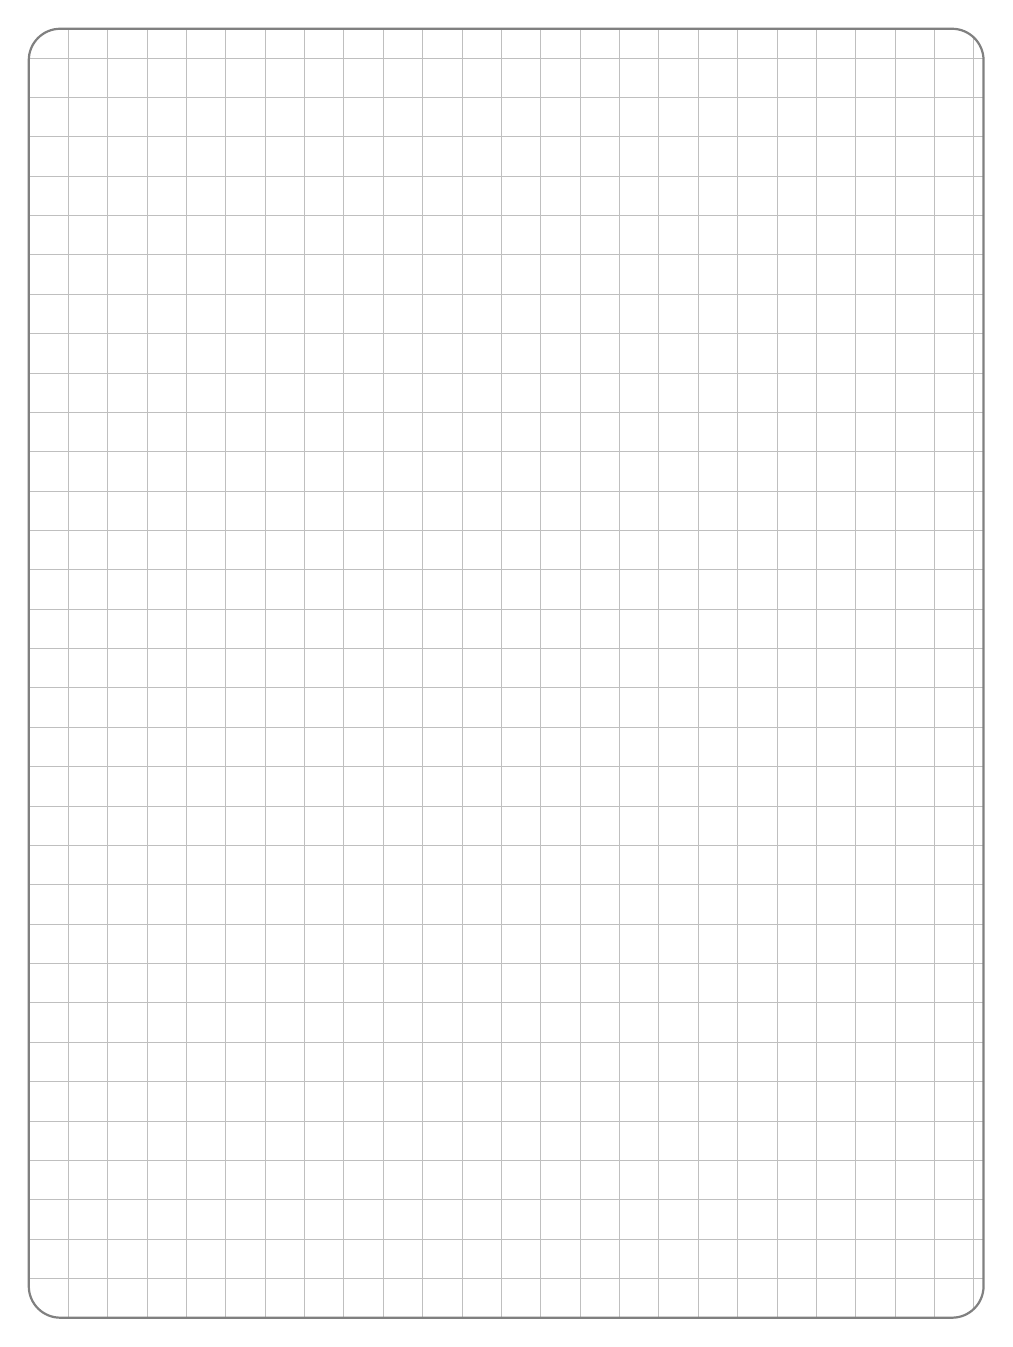
\begin{tikzpicture}
    % параметры
    \def\W{\textwidth}  % ширина прямоугольника
    \def\H{1.35\textwidth}       	% высота прямоугольника
    \def\R{4mm}     	% радиус скругления
    \def\S{5mm}     	% шаг сетки

    % обрезаем всё по прямоугольнику со скруглёнными углами
    \begin{scope}
        \clip[rounded corners=\R] (0,0) rectangle (\W,\H);

        % тетрадная сетка
        \draw[step=\S, very thin, gray!50] (0,0) grid (\W,\H);
    \end{scope}

    % внешний контур
    \draw[rounded corners=\R, line width=0.8pt, gray] (0,0) rectangle (\W,\H);
\end{tikzpicture}
\end{center}

\end{document}